% section: 七つの応用型

\section{七つの応用型}\label{節：応用7パターン}
  ここからは,与えられた\bookterm{recurrence}{漸化式}を四つの基本型へ変える.
  \sectionref{節：漸化式を解く前に}で目指した「きれい」な形へ,使える変形を増やしていこう.

% subsection: 特性方程式型 \, $a_{n+1}=pa_n+q$

\subsection{\texorpdfstring{定数項を消す \, $a_{n+1}=pa_n+q$}{定数項を消す}}\label{節：特性方程式型}
  \bookstep{観察と発想}
  \[
    a_{n+1}=pa_n+q
  \]
  では,定数$q$を取り除けば等比型になる.
  邪魔をしているのは,一定の倍率$p$に加えて毎回$q$が足されることである.
  両辺から$q$を引くだけでは,左辺は$a_{n+1}-q$,右辺は$pa_n$となり,同じ形の量が並ばない.
  左右に同じ形を作るため,各項から引く数をまだ決めずに調整する.
  \sectionref*{節：補助数列の設計}の「同じ更新をする量を引く」方法を使おう.
  以下では$p\ne0,1$を考える.\footnote{ただし$p=1$なら等差型であり,\,$p=0$なら直接$n\ge2$で$a_n=q$と分かる.}

  \bookterm{sequence}{数列}の各項から同じ数$\alpha$を引き,
  \[
    a_{n+1}-\alpha=p(a_n-\alpha)
  \]
  としたい.定数項を合わせると,
  \[
    q-\alpha=-p\alpha
    \quad\Longleftrightarrow\quad
    \alpha=p\alpha+q
  \]
  より$\alpha=\dfrac{q}{1-p}$を得る.更新しても変わらないこの値を\bookterm{fixed}{不動点}という.

  \bookstep{変形と復元}
  元の更新式から\bookterm{fixed}{不動点}の式を引くと,
  \[
    \begin{array}{rrl}
       &a_{n+1}={}&pa_n+q\\
      -\,)&\alpha={}&p\alpha+q\\ \hline
       &a_{n+1}-\alpha={}&p(a_n-\alpha)
    \end{array}
  \]
  となる.$b_n=a_n-\alpha$は公比$p$,初項$a_1-\alpha$の等比型である.
  \bookterm{general}{一般項}を求め,$a_n=b_n+\alpha$へ戻すと,
  \[
    a_n=(a_1-\alpha)p^{n-1}+\alpha.
  \]
  初項が\bookterm{fixed}{不動点}なら,$a_n=\alpha$という定数解になる.

  \noindent\bookblocklink{check-fixed}{problem}{answer}{【確認問題】}\par\nobreak
  \begin{enumerate}[format=\bookitemlink{check-fixed}{problem}{answer}]
    \item $a_{n+1}=3a_n-4$で,何を引くと等比型になるか.
          $a_1=5$と$a_1=2$の場合の\bookterm{general}{一般項}をそれぞれ求めよ.
  \end{enumerate}
  \noindent\bookblocklink{check-fixed}{answer}{problem}{【確認の解答】}\par\nobreak
  \begin{enumerate}[format=\bookitemlink{check-fixed}{answer}{problem}]
    \item $\alpha=3\alpha-4$より$\alpha=2$を引く.
          $a_1=5$なら$a_n=2+3^n$であり,\,$a_1=2$なら$a_n=2$である.
  \end{enumerate}

\noindent \bookblocklink{example-characteristic-1}{problem}{answer}{【例題】}\par\nobreak
\begin{enumerate}[label=(\arabic*),parsep=3pt,format=\bookitemlink{example-characteristic-1}{problem}{answer}]
  \item $\displaystyle a_1=1,\, a_{n+1}=2a_n+1$
  \item $\displaystyle a_1=1,\, a_{n+1}=\frac{1}{2}a_n+2$
  \item $\displaystyle a_1=1,\, a_{n+1}=a_n+2$
\end{enumerate}

\noindent\bookblocklink{example-characteristic-1}{hint}{problem}{【方針】}\par\nobreak
\begin{enumerate}[label=(\arabic*),parsep=3pt,format=\bookitemlink{example-characteristic-1}{hint}{problem}]
  \item まずは,\,$\alpha$を求めて等比型に帰着させる方法で解きましょう.
  \item 同じく,\,$\alpha$を求めて等比型に帰着させる方法で解きましょう.
  \item 等差型として解けます.定数を引く方法では,$\alpha=\alpha+2$を満たす値がないことも確かめましょう.
\end{enumerate}

\noindent\bookblocklink{example-characteristic-1}{answer}{problem}{【解答】}\par\nobreak
\begin{enumerate}[label=(\arabic*),parsep=3pt,format=\bookitemlink{example-characteristic-1}{answer}{problem}]
  \item $\displaystyle a_n=2^n-1$
  \item $\displaystyle a_n=4-3\cdot\left(\frac{1}{2}\right)^{n-1}$
  \item $\displaystyle a_n=1+2(n-1)$
\end{enumerate}

\noindent\bookblocklink{example-characteristic-1}{solution}{problem}{【解法】}\par\nobreak
\begin{enumerate}[label=(\arabic*),parsep=3pt,format=\bookitemlink{example-characteristic-1}{solution}{problem}]
  \item $\alpha=2\alpha+1$より\bookterm{fixed}{不動点}は$-1$である.$b_n=a_n+1$と置くと,
        \[
          \begin{aligned}
            b_{n+1}&=2(a_n+1)=2b_n,\\
            b_1&=2.
          \end{aligned}
        \]
        従って$b_n=2^n$であり,$a_n=b_n-1=2^n-1$となる.
  \item $\alpha=\frac12\alpha+2$より\bookterm{fixed}{不動点}は$4$である.$b_n=a_n-4$と置くと,
        \[
          \begin{aligned}
            b_{n+1}&=\frac12(a_n-4)=\frac12b_n,\\
            b_1&=-3.
          \end{aligned}
        \]
        従って$b_n=-3(\frac12)^{n-1}$であり,$a_n=4-3(\frac12)^{n-1}$となる.
  \item $\alpha=\alpha+2$を満たす値はなく,定数を引く方法は使えない.
        等差型として$a_n=1+2(n-1)$を得る.
\end{enumerate}

\bookstep{グラフと不動点}\label{解釈：不動点と差分}
  定数項を消すために求めた$\alpha$は,更新しても動かない値でもあった.
  今度はこの性質をグラフから見てみよう.
  \bookterm{recurrence}{漸化式}を$a_{n+1}=f(a_n)$と見ると,\bookterm{fixed}{不動点}は$f(\alpha)=\alpha$を満たす.
  つまり,$y=f(x)=px+q$と$y=x$の交点である.

  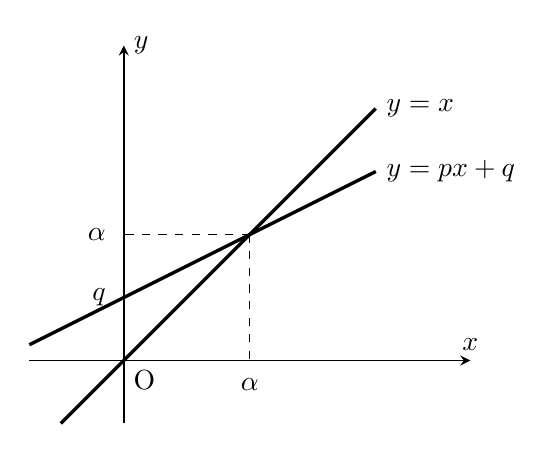
\begin{tikzpicture}[scale=0.8]
    \draw[->,>=stealth,semithick] (-1.5,0)--(5.5,0)node[above]{$x$};
    \draw[->,>=stealth,semithick] (0,-1)--(0,5)node[right]{$y$};
    \draw (0,0)node[below right]{O};

    \draw[very thick,domain=-1:4]
      plot(\x,\x)node[right]{$y=x$};

    \draw[very thick,domain=-1.5:4]
      plot(\x,\x/2+1) node[right] {$y=px+q$};

    % q
    \node[left=3pt] at (0,1) {$q$};

    % 交点から各軸へ点線
    \draw[dashed] (2,2) -- (2,0);
    \draw[dashed] (2,2) -- (0,2);

    % α
    \node[below=3pt] at (2,0) {$\alpha$};
    \node[left=3pt] at (0,2) {$\alpha$};
  \end{tikzpicture}
  \begin{center}
    \BookFigureCaption{直線の交点として捉える\bookterm{fixed}{不動点}}
  \end{center}

  この交点$(\alpha,\alpha)$を新しい原点にする.
  新しい原点からの座標で表すと,定数を引く式変形が座標の取り方として見える.
  $X=x-\alpha,\ Y=y-\alpha$と置くと,$\alpha=p\alpha+q$より二つの直線は$Y=pX$と$Y=X$になる.
  $x$座標と$y$座標の両方から$\alpha$を引くことが,等比型への変形に対応している.

  不動点からのずれは$p$倍される.\footnote{$p<0$ではずれの符号が交互に変わる.$p=-1$では,$a_1\ne\alpha$なら二つの値を往復する.$p=1$の等差型と$p=0$の場合は節の冒頭で分けた.}%
  初項が$\alpha$なら定数解,異なるなら$|p|>1$でずれが増大し,$|p|<1$で$0$へ近づく.
  後者では$a_n\to\alpha$となる.例題(2)が$4$へ近づくのはこのためである.

\bookstep{階差を取って定数項を消す}
  同じ$q$を消すには,隣り合う二つの更新式を引く方法もある.
  \begin{align*}
    &a_{n+1}=pa_n+q \booktag{affine-difference-1}{1}\\
    &a_{n+2}=pa_{n+1}+q \booktag{affine-difference-2}{2}\\
  \end{align*}
  $\bookeqbackref{affine-difference-2}{(2)}-\bookeqbackref{affine-difference-1}{(1)}$をし
  \[
    a_{n+2}-a_{n+1}=p(a_{n+1}-a_n)
  \]
  ここで,$d_n=a_{n+1}-a_n$と置くと,
  \[
    d_{n+1}=pd_n,\qquad d_1=(p-1)a_1+q
  \]
  となる.等比型になった\textbf{階差}$d_n=d_1p^{n-1}$を,\sectionref*{節：階差型}と同じように足し戻す.
  \begin{align*}
    a_n&=a_1+\sum_{k=1}^{n-1}d_k\\
       &=a_1+d_1\frac{p^{n-1}-1}{p-1}\\
       &=\alpha+(a_1-\alpha)p^{n-1}
  \end{align*}
  $d_1=(p-1)(a_1-\alpha)$より,不動点を引く方法と一致する.
  $p=1$の場合も階差は一定なので,$a_n=a_1+(n-1)q$と足し戻せる.

  二つの直線$y=px$と$y=px+q$の差は$q$である.一方,更新式どうしの引き算では異なる入力を比べる.
  $f(x)=px+q$なら,
  \[
    f(x)-f(y)=(px+q)-(py+q)=p(x-y)
  \]
  となる.$x=a_{n+1},\ y=a_n$としたものが\bookeqref{affine-difference-2}{(2)}から\bookeqref{affine-difference-1}{(1)}を引いた式である.\footnote{添字を一つずらして引く操作は,付録\sectionref{節：差分から始まる離散的な微積分}で扱う\bookterm{difference-operator}{差分}の考え方につながる.}
  共通の$q$が消えた.二つの直線も確認しよう.

  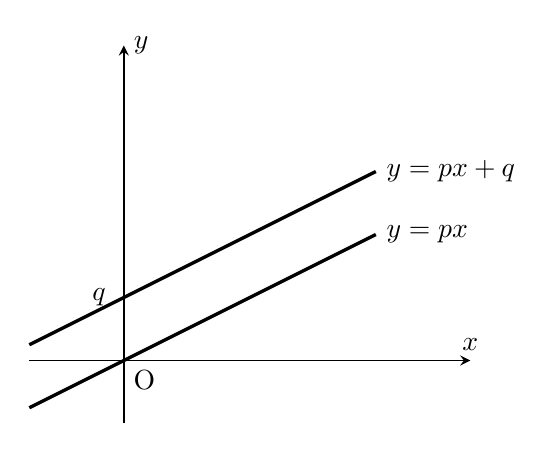
\begin{tikzpicture}[scale=0.8]
    \draw[->,>=stealth,semithick] (-1.5,0)--(5.5,0)node[above]{$x$};
    \draw[->,>=stealth,semithick] (0,-1)--(0,5)node[right]{$y$};
    \draw (0,0)node[below right]{O};

    \draw[very thick,domain=-1.5:4]
      plot(\x,\x/2)node[right]{$y=px$};

    \draw[very thick,domain=-1.5:4]
      plot(\x,\x/2+1) node[right] {$y=px+q$};

    % q
    \node[left=3pt] at (0,1) {$q$};

  \end{tikzpicture}
  \begin{center}
    \BookFigureCaption{定数項の違いを表す平行な直線}
  \end{center}

  不動点からのずれと隣り合う項の差は,同じ定数項を消す二つの見方である.
  この先では引く量が一次式などへ広がり,二項をまとめる際には倍率を求める\mbox{\bookterm{characteristic}{特性方程式}}が現れる.
  今の$\alpha$は変わらない値,後の根は更新の倍率である.付録の\bookterm{matrix}{行列}でもつながりを見直す.

% subsection: 階差等比複合型 \, $\displaystyle a_{n+1}=pa_n+f(n)$

\subsection{\texorpdfstring{多項式・指数の付加項 \, $\displaystyle a_{n+1}=pa_n+f(n)$}{多項式・指数の付加項}}\label{節：階差等比複合型}
  \begin{bookpoint}
    \textbf{共通の付加項を消す}\par
    付加項が$n$の多項式なら,$a_n$から多項式を引いて等比型にする.付加項が$q^n$なら,$q$の累乗で割る方法も試せる.
  \end{bookpoint}
  \subsubsection{\texorpdfstring{多項式を引く \, $\displaystyle a_{n+1}=pa_n+f(n)$}{多項式を引く}}
    \sectionref*{節：特性方程式型}では,各項から定数を引いて等比型にした.
    今回は付加項$f(n)$が$n$によって変わるため,引く量も$n$によって変えてみる.
    補助数列$b_n=a_n-g(n)$が等比型になるように,引く式$g(n)$を決めよう.
    $f(n)$を多項式とし,$p\ne1$を考えよう.$p=1$なら\bookterm{difference}{階差}型である.

    \bookstep{引く量を選ぶ}
    $b_n=a_n-g(n)$を等比型にするための条件は
    \[
      g(n+1)=pg(n)+f(n)
    \]
    である.この条件なら,
    \[
      \begin{array}{rrl}
        &a_{n+1}={}&pa_n+f(n)\\
        -\,)&g(n+1)={}&pg(n)+f(n)\\ \hline
        &a_{n+1}-g(n+1)={}&p\{a_n-g(n)\}
      \end{array}
    \]
    となり,付加項が消える.
    $a_n=g(n)+b_n$は,\sectionref*{節：非同次と解の組合せ}の「既知の解と\bookterm{homogeneous}{同次}の解」の分解である.
    $g(n)$を探し,$b_n$を\bookterm{initial}{初期条件}から決める.

    まず$a_{n+1}=2a_n+n-1$で試してみよう.
    付加項が一次式なので,引く量も$g(n)=un+v$と置く.
    一次式は添字を一つずらしても一次式のままである.
    元の付加項と次数をそろえ,未知の係数$u,v$で残る項を消そう.
    条件$g(n+1)=2g(n)+n-1$に代入すると,
    \[
      un+u+v=(2u+1)n+2v-1
    \]
    となる.すべての$n\ge1$で成り立つよう係数を合わせると,
    \[
      u=2u+1,\qquad u+v=2v-1
    \]
    より$u=-1,\ v=0$,すなわち$g(n)=-n$を得る.
    従って
    \[
      a_{n+1}+(n+1)=2(a_n+n)
    \]
    となる.初項$a_1+1$から,
    \[
      a_n=(a_1+1)2^{n-1}-n
    \]
    と元へ戻せる.この例は\bookproblemref{practice-basic}{4}{標準問4}でも扱う.

    \bookstep{多項式へ広げる}
    同じ手順を,$f(n)$が$m$次式の場合に広げよう.
    $p\ne1$のときは$m$次の多項式
    \[
      g(n)=x_0+x_1n+\cdots+x_mn^m
    \]
    を候補にする.$g(n+1)-pg(n)$の最高次の係数は$(1-p)x_m$である.
    これを$f(n)$の最高次の係数に合わせ,次に一段低い係数を合わせる.
    $1-p\ne0$なので,この順に$x_m,x_{m-1},\ldots,x_0$を決められる.\footnote{未知の係数を比較して求めるこの方法を\bookterm{undetermined}{未定係数法}という.}

    \bookstep{一般項を求める}
    $b_{n+1}=pb_n$を解き,\,$a_n=b_n+g(n)$へ戻す.
    $p\ne0,1$なら
    \[
      a_n=\{a_1-g(1)\}p^{n-1}+g(n)
    \]
    となる.\footnote{$p=0$なら初項を別に扱い,$n\ge2$で$a_n=f(n-1)$と直接求める.}
    一方,\,$p=1$で$f(n)$が$m$次なら,$g(n+1)-g(n)=f(n)$を満たす多項式$g(n)$は$m+1$次になる.
    例えば$a_{n+1}=a_n+n$では,\,$g(n)=\frac{n(n-1)}2$が同じ更新を満たす.

  \subsubsection{\texorpdfstring{指数で割る  \, $\displaystyle a_{n+1}=pa_n+q^n$}{指数で割る}}
    $a_{n+1}=pa_n+q^n$では,$q$の累乗で割ると付加項が定数になる.$q\ne0$とする.\footnote{$q=0$なら$n\ge1$で$q^n=0$なので等比型になる.}
    付加項$q^n$を$1$にするために,両辺を$q^n$で割る.
    左辺の添字は$n+1$なので,それに合わせて第$n$項を割る量は$q^{n-1}$とする.
    両辺を$q^n$で割り,$b_n=\dfrac{a_n}{q^{n-1}}$と置くと,
    \[
      \begin{aligned}
        \frac{a_{n+1}}{q^n}&=\frac pq\frac{a_n}{q^{n-1}}+1,\\
        b_{n+1}&=\frac pq b_n+1.
      \end{aligned}
    \]
    \booknavref{節：特性方程式型}{定数項を消す方法}へ戻った.
    ただし$p=q$のときは$b_{n+1}=b_n+1$(\bookterm{arithmetic}{等差数列})になり,\bookterm{fixed}{不動点}$\alpha$が存在しない.\footnote{\bookproblemref{example-characteristic-1}{3}{先ほどの例題(3)}と同じ状況である.}
    この場合は$b_n=b_1+(n-1)$として直接求まる.
    いずれの場合も,求めた$b_n$に$q^{n-1}$を掛ければ元の$a_n$に戻る.
    例えば$a_1=1,\,a_{n+1}=2a_n+2^n$(\,$p=q=2$)ならば$b_n=\dfrac{a_n}{2^{n-1}}$が\bookterm{arithmetic}{等差数列}となり,\,$a_n=n\cdot2^{n-1}$が得られる.

% subsection: 対数型 \, $a_{n+1}=pa_n^q$

\subsection{\texorpdfstring{対数型 \, $a_{n+1}=pa_n^q$}{対数型}}\label{節：対数型}
  \begin{bookpoint}
    \textbf{積と冪をほどく}\par
    \bookterm{logarithm}{対数}を取る発想は指数の扱いを簡単にするためである.実数の\bookterm{logarithm}{対数}を使う前に,項や底の条件を確認する.
  \end{bookpoint}
  \noindent\textbf{【観察と発想】}\par
  \sectionref*{節：指数対数}の公式$\log_t(x^q)=q\log_t x$で,指数を係数にできる.
  積・商・累乗を和・差・定数倍へ変えるために,正値を確認して\bookterm{logarithm}{対数}を取ろう.

  \[
    a_{n+1}=pa_n^q
  \]
  ただし,$p>0,\,a_1>0$とする. このとき,すべての項が正となり,\bookterm{logarithm}{対数}を取ることができる.\footnote{$a_n>0$ならば$p a_n^q>0$であるから,\bookterm{induction}{数学的帰納法}によりすべての項が正となり,\bookterm{logarithm}{対数}を取ることができる.}
  まず,$p\ne1$の場合を考え,$p$を\bookterm{logarithm}{対数}の底に選ぶ.
  この式について,両辺の\bookterm{logarithm}{対数}を取ると
  \[
    \begin{aligned}
      \log_pa_{n+1}&=\log_pp+q\log_pa_n\\
                  &=q\log_pa_n+1.
    \end{aligned}
  \]
  $b_n=\log_pa_n$なら$b_{n+1}=qb_n+1$である.
  $q\ne1$ならば不動点を引いて定数項を消すことができる.
  $q=1$のときは$b_{n+1}=b_n+1$という等差型となり,$a_n=a_1p^{n-1}$を得る.
  また,$p=1$のときは$p$を\bookterm{logarithm}{対数}の底にできないが,底を$2$などに選べば
  \[
    b_n=\log_2a_n,\qquad b_{n+1}=qb_n
  \]
  となり,$q\ne0$ならば$a_n=a_1^{q^{n-1}}$を得る.
  $q=0$の場合は$a_1$を別に扱い,$n\ge2$では$a_n=1$である.
  底は正で$1$以外なら自由である.整数$m$で$p=k^m$と書けるなら,$k$を底にすると$\log_kp=m$となり,定数を整数にできる.
  例題(2)では商を差に変え,逆数の更新を符号反転として追う.

  \noindent\bookblocklink{example-logarithmic-1}{problem}{answer}{【例題】}\par\nobreak
  \begin{enumerate}[label=(\arabic*),parsep=3pt,format=\bookitemlink{example-logarithmic-1}{problem}{answer}]
    \item $\displaystyle a_1=2,\quad a_{n+1}=2a_n^2$
    \item $\displaystyle a_1=\frac{1}{2},\quad a_{n+1}=\frac{1}{a_n}$
    \item $\displaystyle a_1=1,\quad a_{n+1}=2^na_n$
    \item $\displaystyle a_1=5,\quad a_{n+1}=a_n^2-2a_n+2$
    \item $\displaystyle a_1=2,\quad a_{n+1}=\frac{a_n^2}{2^n}$
    \item $\displaystyle a_1=1,\quad a_{n+1}=(n+1)a_n$
  \end{enumerate}

  \noindent\bookblocklink{example-logarithmic-1}{hint}{problem}{【方針】}\par\nobreak
  \begin{enumerate}[label=(\arabic*),parsep=3pt,format=\bookitemlink{example-logarithmic-1}{hint}{problem}]
    \item $b_n=\log_2a_n$で$b_{n+1}=2b_n+1$に変え,定数項を消します.
    \item 逆数を\bookterm{logarithm}{対数}で符号反転に変えます.
    \item $f(n)=2^n$が指数関数なので,\bookterm{logarithm}{対数}を取ると和の形に帰着できます.
    \item \bookterm{square}{平方完成}で$a_{n+1}-1=(a_n-1)^2$を作ります.\bookterm{logarithm}{対数}を取る量は$a_n$ではなく$a_n-1$であり,その正値を先に確認します.
    \item $b_n=\log_2a_n$から一次式$n+1$を引くと等比型になります.
    \item 積を直接まとめる方法と,\bookterm{logarithm}{対数}で和に変える方法を比べましょう.最後には同じ積$n!$を計算します.
  \end{enumerate}

  \noindent\bookblocklink{example-logarithmic-1}{answer}{problem}{【解答】}\par\nobreak
  \begin{enumerate}[label=(\arabic*),parsep=3pt,format=\bookitemlink{example-logarithmic-1}{answer}{problem}]
    \item $\displaystyle a_n=2^{2^{n}-1}$
    \item $a_n=2^{(-1)^{n}}$
    \item $a_n=2^{\frac{n(n-1)}{2}}$
    \item $a_n=2^{2^n}+1$
    \item $\displaystyle a_n=2^{\,n+1-2^{n-1}}$
    \item $a_n=n!$
  \end{enumerate}

  \noindent\bookblocklink{example-logarithmic-1}{solution}{problem}{【解法】}\par\nobreak

  (1),(2),(3),(5),(6)は初項が正で,正の項から次も正になる.\bookterm{induction}{数学的帰納法}より全項が正である.
  (4)は$a_1-1=4>0$と$a_{n+1}-1=(a_n-1)^2$から,$a_n-1>0$を保つ.この量に\bookterm{logarithm}{対数}を取る.
  \begin{enumerate}[label=(\arabic*),parsep=3pt,format=\bookitemlink{example-logarithmic-1}{solution}{problem}]
    \item $b_n=\log_2a_n$と置くと,
          \[
            b_{n+1}=2b_n+1,\qquad b_1=1.
          \]
          $b_n+1$は初項$2$,公比$2$の等比型なので,
          \[
            b_n+1=2^n,\qquad a_n=2^{b_n}=2^{2^n-1}.
          \]
    \item $b_n=\log_2a_n$と置くと,逆数は
          \[
            b_{n+1}=-b_n,\qquad b_1=\log_2\frac12=-1
          \]
          に変わる.従って$b_n=(-1)^n$であり,$a_n=2^{(-1)^n}$となる.
    \item 自然\bookterm{logarithm}{対数}を取れば$\log a_{n+1}=\log a_n+n\log2$である.差を足すと,
          \[
            \log a_n=\sum_{k=1}^{n-1}k\log2=\frac{n(n-1)}2\log2.
          \]
          従って$a_n=2^{n(n-1)/2}$となる.
    \item \bookterm{square}{平方完成}で$a_{n+1}-1=(a_n-1)^2$となる.\bookterm{logarithm}{対数}を取ると,
          \[
            \log_2(a_{n+1}-1)=2\log_2(a_n-1).
          \]
          初項は$\log_2(a_1-1)=2$だから,$\log_2(a_n-1)=2^n$であり,$a_n=2^{2^n}+1$となる.
    \item $b_n=\log_2a_n$と置くと,$b_{n+1}=2b_n-n,\ b_1=1$である.
          一次式$n+1$を引けば,
          \[
            b_{n+1}-(n+2)=2\{b_n-(n+1)\}.
          \]
          $c_n=b_n-(n+1)$は$c_{n+1}=2c_n,\ c_1=-1$を満たすので,
          \[
            c_n=-2^{n-1},\quad b_n=n+1-2^{n-1}.
          \]
          戻すと$a_n=2^{\,n+1-2^{n-1}}$となる.
    \item 自然\bookterm{logarithm}{対数}を取れば$\log a_{n+1}=\log a_n+\log(n+1)$である.
          \[
            \log a_n=\log1+\log2+\cdots+\log n=\log n!.
          \]
          従って$a_n=n!$となる.直接積を取っても同じ結果が得られる.
  \end{enumerate}
  \noindent\textbf{【補足】}

  (3),(6)の$\log$は底が$e$の自然\bookterm{logarithm}{対数}である.
  変形後の真数が$0$や負なら,実数の\bookterm{logarithm}{対数}は取れない.例えば(4)で初項が$1$なら定数\bookterm{sequence}{数列}$a_n=1$となり,$\log(a_n-1)$を取らずに扱う.

  \noindent\bookblocklink{check-log-domain}{problem}{answer}{【確認問題】}\par\nobreak
  \begin{enumerate}[format=\bookitemlink{check-log-domain}{problem}{answer}]
    \item $a_{n+1}=a_n^2$で,初項が$2,0,-2$の場合を比較せよ.
          最初から実数の\bookterm{logarithm}{対数}を取れるのはどの場合か.取れない場合にも\bookterm{sequence}{数列}は定義されるか.
  \end{enumerate}
  \noindent\bookblocklink{check-log-domain}{answer}{problem}{【確認の解答】}\par\nobreak
  \begin{enumerate}[format=\bookitemlink{check-log-domain}{answer}{problem}]
    \item 初項$2$ならすべての項が正である.
          初項$0$なら零列,初項$-2$なら第2項以降が正である.
          いずれも元の\bookterm{recurrence}{漸化式}は定義される.\bookterm{logarithm}{対数}を取る条件と,元の\bookterm{sequence}{数列}が存在する条件は区別する.
  \end{enumerate}

% parent file: 分数型
\subsection{分数型}\label{節：分数型}
\begin{bookpoint}
  \textbf{分母を簡単にする}\par
  逆数,または\bookterm{fixed}{不動点}からの二つの差の比を追う.
  分母が零になる初期値と定数解の分岐を確かめてから,置き換えを使う.
\end{bookpoint}
% subsubsection: 逆数型  \, $\displaystyle a_{n+1}=\frac{pa_n}{qa_n+r}$

\subsubsection{\texorpdfstring{逆数型  \, $\displaystyle a_{n+1}=\frac{pa_n}{qa_n+r}$}{逆数型}}\label{節：逆数型}
    分子が$a_n$の定数倍である\bookterm{recurrence}{漸化式}を考えよう.
    逆数を取れば,分母にあった一次式を$a_n$で割り,定数と$\frac1{a_n}$の和に分けられる.
    以下では,$p\ne0$かつ$a_n\ne0$であり,$qa_n+r\ne0$として議論する.\footnote{$a_1=0$は逆数を取る前に分ける.$r\ne0$ならすべての項が$0$となる.$r=0$なら最初の更新から分母が$0$となり,そのままでは定義できない.}
    両辺の逆数を取り,$b_n=1/a_n$と置くと,
    \begin{align*}
      \frac{1}{a_{n+1}}&=\frac{qa_n+r}{pa_n}
        =\frac{q}{p}+\frac{r}{p}\cdot\frac{1}{a_n},\\
      b_{n+1}&=\frac{r}{p}b_n+\frac{q}{p}
    \end{align*}
    ここから定数項を消す型または等差型として$b_n$を求め,最後に$a_n=1/b_n$へ戻す.
    ただし$b_n=0$となる項は逆数を戻せないため,元の漸化式が定義されるかも確認する.

    \noindent \bookblocklink{example-reciprocal-1}{problem}{answer}{【例題】}\par\nobreak
    \begin{enumerate}[label=(\arabic*),parsep=3pt,format=\bookitemlink{example-reciprocal-1}{problem}{answer}]
      \item $\displaystyle a_1=1,\, a_{n+1}=\frac{a_n}{a_n+1}$
      \item $\displaystyle a_1=1,\, a_{n+1}=\frac{-a_n}{2a_n+1}$
    \end{enumerate}

    \noindent\bookblocklink{example-reciprocal-1}{hint}{problem}{【方針】}\par\nobreak
    \begin{enumerate}[label=(\arabic*),parsep=3pt,format=\bookitemlink{example-reciprocal-1}{hint}{problem}]
      \item 逆数を取ると,$1/a_n$が毎回$1$ずつ増える形になります.
      \item 逆数を取って一次の\bookterm{recurrence}{漸化式}に帰着させましょう.
    \end{enumerate}

    \noindent\bookblocklink{example-reciprocal-1}{answer}{problem}{【解答】}\par\nobreak
    \begin{enumerate}[label=(\arabic*),parsep=3pt,format=\bookitemlink{example-reciprocal-1}{answer}{problem}]
      \item $\displaystyle a_n=\frac{1}{n}$
      \item $\displaystyle a_n=\frac{1}{2(-1)^{n-1}-1}$
    \end{enumerate}

    \noindent\bookblocklink{example-reciprocal-1}{solution}{problem}{【解法】}\par\nobreak
    \begin{enumerate}[label=(\arabic*),parsep=3pt,format=\bookitemlink{example-reciprocal-1}{solution}{problem}]
      \item $\displaystyle a_1=1,\, a_{n+1}=\frac{a_n}{a_n+1}$\\
            正の項と分母が続くので,逆数を取れる.$b_n=1/a_n$と置くと,
            \begin{align*}
              &\frac{1}{a_{n+1}}=1+\frac{1}{a_n},\\
              &b_{n+1}=b_n+1,\quad b_1=1\\
              &\therefore \quad b_n=n,\quad a_n=\frac1n
            \end{align*}
      \item $\displaystyle a_1=1,\, a_{n+1}=\frac{-a_n}{2a_n+1}$\\
            初めの更新は$1\longmapsto-1/3\longmapsto1$となる.
            項も分母も零でないので,$b_n=1/a_n$と置くと,
            \begin{align*}
              &\frac{1}{a_{n+1}}=-2-\frac{1}{a_n},\\
              &b_{n+1}=-b_n-2,\quad b_1=1
            \end{align*}
            \bookterm{fixed}{不動点}は$-1$なので,$c_n=b_n+1$と置き,定数項を消す.
            \begin{align*}
              &c_{n+1}=-c_n,\quad c_1=2\\
              &\therefore \quad b_n=c_n-1=2(-1)^{n-1}-1,\\
              &a_n=\frac{1}{2(-1)^{n-1}-1}
            \end{align*}
    \end{enumerate}

% subsubsection: 1次分数型  \, $\displaystyle a_{n+1}=\frac{pa_n+q}{ra_n+s}$

\subsubsection{\texorpdfstring{一次分数型  \, $\displaystyle a_{n+1}=\frac{pa_n+q}{ra_n+s}$}{一次分数型}}\label{節：1次分数型}
    分子にも定数項がある\bookterm{recurrence}{漸化式}を考えよう.
    以下では$r\ne0$, $ps-qr\ne0$とし,元の分母が$0$にならない範囲で議論する.\footnote{$r=0,\ s\ne0$なら定数項を消す型へ戻る.
    $r\ne0,\ ps-qr=0$なら,分母が非零の入力に対して右辺は定数$p/r$になる.次の分母も確認する.例えば$(a_n-1)/(a_n-1)$は,初項が$1$でなくても次項が$1$になり,次の更新は定義できない.}
    分子の定数項$q$を消せれば,逆数型として解ける.

    \bookstep{一つの差を追う}
    \sectionref{節：特性方程式型}と同じく,各項から定数を引いてみよう.
    $u_n=a_n-\alpha$と置き,分子の定数項が消えるように$\alpha$を選ぶ.
    $a_n=u_n+\alpha$を代入すると,
    \BookMathLayout{\begin{align*}
      u_{n+1}&=\frac{p(u_n+\alpha)+q}{r(u_n+\alpha)+s}-\alpha\\
      &=\frac{(p-r\alpha)u_n+p\alpha+q-r\alpha^2-s\alpha}
        {ru_n+r\alpha+s}
    \end{align*}}{\[
      \begin{aligned}
        &u_{n+1}\\
        &{}=\frac{p(u_n+\alpha)+q}{r(u_n+\alpha)+s}-\alpha\\
        &{}=\frac{(p-r\alpha)u_n+p\alpha+q-r\alpha^2-s\alpha}
          {ru_n+r\alpha+s}
      \end{aligned}
    \]}
    従って,
    \[
      r\alpha^2+(s-p)\alpha-q=0
      \quad\Longleftrightarrow\quad
      \alpha=\frac{p\alpha+q}{r\alpha+s}
    \]
    を満たす$\alpha$,すなわち元の\bookterm{fixed}{不動点}を引けば,
    \[
      u_{n+1}=\frac{(p-r\alpha)u_n}{ru_n+r\alpha+s}
    \]
    という逆数型になる.ここで,$p-r\alpha$も$r\alpha+s$も零でない.\footnote{不動点の方程式より,$(p-r\alpha)(r\alpha+s)=ps-qr\ne0$.}
    初項が$\alpha$なら定数列である.それ以外では$u_n$は途中で零にならず,逆数を取って解ける.

    \bookstep{二つの差の比を追う}
    不動点の方程式
    \[
      rx^2+(s-p)x-q=0
    \]
    が異なる二つの実数解$\alpha,\beta$を持つとしよう.
    どちらも定数項を消せるので,先ほどの変形を$a_n$で書けば,
    \begin{align*}
      a_{n+1}-\alpha
      &=\frac{p-r\alpha}{ra_n+s}(a_n-\alpha),\\
      a_{n+1}-\beta
      &=\frac{p-r\beta}{ra_n+s}(a_n-\beta)
    \end{align*}
    となる.倍率に$a_n$が含まれるため,各々の差は一般には\bookterm{geometric}{等比数列}にならない.
    しかし,\textbf{二つの式の比を取れば,共通の分母が消える}.

    初項が$\alpha$または$\beta$なら定数\bookterm{sequence}{数列}として分けておく.
    それ以外では,$p-r\beta\ne0$なので,$a_n\ne\beta$から$a_{n+1}\ne\beta$が続く.
    従って,差の比を取れる.
    \begin{align*}
      \frac{a_{n+1}-\alpha}{a_{n+1}-\beta}
      &=\frac{p-r\alpha}{p-r\beta}
        \frac{a_n-\alpha}{a_n-\beta}
    \end{align*}
    ここで$b_n=(a_n-\alpha)/(a_n-\beta)$と置けば,
    \[
      b_{n+1}=\frac{p-r\alpha}{p-r\beta}b_n
    \]
    となる.一つの差を逆数型として解く代わりに,二つの差の比を直接等比型にできた.\footnote{二つの解のどちらを$\alpha,\beta$と名付けてもよい.}
    初項$b_1=(a_1-\alpha)/(a_1-\beta)$を用いて,
    \[
      b_n=\frac{a_1-\alpha}{a_1-\beta}\left(\frac{p-r\alpha}{p-r\beta}\right)^{n-1} \booktag{mobius-geometric}{＊}
    \]
    を得る.

    \bookstep{元の項へ戻す}
    $b_n(a_n-\beta)=a_n-\alpha$を$a_n$について解くと,
    \[
      a_n=\frac{\beta b_n-\alpha}{b_n-1}
    \]
    となる.有限の$a_n$では$\alpha\ne\beta$より$b_n\ne1$なので,この割り算ができる.
    \bookeqbackref{mobius-geometric}{(＊)}を代入すればよい.
    逆に,公式上で$b_n=1$となる項は復元できず,元の更新をそこまで定義できない.

    不動点の方程式が重解$\alpha$を持つ場合は,異なる差を作れない.
    一つの差$u_n=a_n-\alpha$に戻り,逆数を取れば等差型になる.
    例題(3)で計算し,例題の後で一般の係数でも確かめよう.

    \noindent \bookblocklink{example-mobius-1}{problem}{answer}{【例題】}\par\nobreak
    \begin{enumerate}[label=(\arabic*),parsep=3pt,format=\bookitemlink{example-mobius-1}{problem}{answer}]
      \item $\displaystyle a_1=3,\, a_{n+1}=\frac{2a_n+1}{a_n+2}$
      \item $\displaystyle a_1=0,\, a_{n+1}=\frac{a_n+4}{a_n+1}$
      \item $\displaystyle a_1=5,\, a_{n+1}=\dfrac{4a_{n}-9}{a_{n}-2}$
      \item $\displaystyle a_1=1,\, a_{n+1}=1+\frac{1}{a_n}$
    \end{enumerate}

    \noindent\bookblocklink{example-mobius-1}{hint}{problem}{【方針】}\par\nobreak
    \begin{enumerate}[label=(\arabic*),parsep=3pt,format=\bookitemlink{example-mobius-1}{hint}{problem}]
      \item 不動点$1,-1$からの差の比を作ると,共通の分母$a_n+2$が消えます.
      \item 同様に\bookterm{fixed}{不動点}$\alpha,\beta$を求めましょう.今回は片方が負の値になります.
      \item 今回は\bookterm{fixed}{不動点}の方程式が重解になります.\,$\dfrac{a_n-\alpha}{a_n-\beta}$は使えないので,\,$b_n=a_n-\alpha$と置いてから逆数型に帰着させる別の手法を使います.
      \item このような形も一次分数型です.解と係数の関係を活用して解きましょう.
    \end{enumerate}

    \noindent\bookblocklink{example-mobius-1}{answer}{problem}{【解答】}\par\nobreak
    \begin{enumerate}[label=(\arabic*),parsep=3pt,format=\bookitemlink{example-mobius-1}{answer}{problem}]
      \item $\displaystyle a_n=\frac{2\cdot3^{n-1}+1}{2\cdot3^{n-1}-1}$
      \item $\displaystyle a_n=\frac{2\left(3^{n-1}+(-1)^n\right)}{3^{n-1}-(-1)^n}$
      \item $a_{n}=\dfrac{6n-1}{2n-1}$
      \item $\displaystyle a_n=\cfrac{\left(\cfrac{1-\sqrt{5}}{2}\right)^{n+1}-\left(\cfrac{1+\sqrt{5}}{2}\right)^{n+1}}{\left(\cfrac{1-\sqrt{5}}{2}\right)^n-\left(\cfrac{1+\sqrt{5}}{2}\right)^n}$
    \end{enumerate}

    \noindent\bookblocklink{example-mobius-1}{solution}{problem}{【解法】}\par\nobreak
    \begin{enumerate}[label=(\arabic*),parsep=3pt,format=\bookitemlink{example-mobius-1}{solution}{problem}]
      \item $\displaystyle a_1=3,\, a_{n+1}=\frac{2a_n+1}{a_n+2}$\\
            \bookterm{fixed}{不動点}の方程式$x=(2x+1)/(x+2)$の解は$1,-1$である.
            $b_n=(a_n-1)/(a_n+1)$と置くと,
            \begin{align*}
              b_{n+1}&=\cfrac{\cfrac{2a_n+1}{a_n+2}-1}{\cfrac{2a_n+1}{a_n+2}+1}\\
              &=\frac{2a_n+1-(a_n+2)}{2a_n+1+(a_n+2)}\\
              &=\frac13\frac{a_n-1}{a_n+1}=\frac13b_n
            \end{align*}
            $b_1=(3-1)/(3+1)=1/2$なので,
            \[
              b_n=\frac12\left(\frac13\right)^{n-1}
                =\frac1{2\cdot3^{n-1}}
            \]
            である.元の項への復元は,
            \begin{align*}
              b_n(a_n+1)&=a_n-1,\\
              a_n&=\frac{1+b_n}{1-b_n}
                =\frac{2\cdot3^{n-1}+1}{2\cdot3^{n-1}-1}
            \end{align*}
            となる.
      \item $\displaystyle a_1=0,\, a_{n+1}=\frac{a_n+4}{a_n+1}$\\
            \bookterm{fixed}{不動点}の方程式$x=(x+4)/(x+1)$の解は$2,-2$である.
            倍率は$(1-2)/(1+2)=-1/3$なので,$b_n=(a_n-2)/(a_n+2)$と置くと,
            \begin{align*}
              b_{n+1}&=-\frac13b_n,\quad b_1=-1,\\
              b_n&=(-1)\left(-\frac13\right)^{n-1}
                =\frac{(-1)^n}{3^{n-1}}
            \end{align*}
            を得る.$b_n(a_n+2)=a_n-2$から復元して,
            \begin{align*}
              a_n&=\frac{2(1+b_n)}{1-b_n}\\
              &=\frac{2\left(3^{n-1}+(-1)^n\right)}{3^{n-1}-(-1)^n}
            \end{align*}
            となる.
      \item $\displaystyle a_1=5,\, a_{n+1}=\dfrac{4a_n-9}{a_n-2}$\\
            \bookterm{fixed}{不動点}の方程式$x=(4x-9)/(x-2)$は重解$3$を持つ.
            $b_n=a_n-3$と置くと,
            \begin{align*}
              b_{n+1}&=\frac{4a_n-9}{a_n-2}-3
                =\frac{a_n-3}{a_n-2}\\
              &=\frac{b_n}{b_n+1},\quad b_1=2
            \end{align*}
            となる.正の$b_n$が続くので,$b_n$も元の分母$b_n+1$も零でない.
            逆数を取れば,
            \begin{align*}
              \frac1{b_{n+1}}&=\frac1{b_n}+1,\\
              \frac1{b_n}&=\frac12+(n-1)=\frac{2n-1}{2}
            \end{align*}
            である.従って,
            \[
              a_n=3+b_n=3+\frac2{2n-1}=\frac{6n-1}{2n-1}
            \]
            を得る.
      \item $\displaystyle a_1=1,\, a_{n+1}=1+\frac1{a_n}$\\
            右辺を$(a_n+1)/a_n$と書けば,一次分数型である.
            \bookterm{fixed}{不動点}の方程式
            \[
              x=\frac{x+1}{x}\booktag{mobius-example-fixed}{1}
            \]
            の解を
            \[
              \alpha=\frac{1+\sqrt5}{2},\qquad
              \beta=\frac{1-\sqrt5}{2}
            \]
            とする.\bookeqbackref{mobius-example-fixed}{(1)}の解と係数の関係から,
            \[
              \alpha+\beta=1,\qquad \alpha\beta=-1
                \booktag{mobius-example-roots}{2}
            \]
            である.$b_n=(a_n-\alpha)/(a_n-\beta)$と置くと,
            \begin{align*}
              b_{n+1}&=\frac{a_n+1-\alpha a_n}{a_n+1-\beta a_n}\\
              &=\frac{(1-\alpha)a_n+1}{(1-\beta)a_n+1}
                \booktag{mobius-example-ratio}{3}
            \end{align*}
            となる.\bookeqbackref{mobius-example-roots}{(2)}を\bookeqbackref{mobius-example-ratio}{(3)}に使えば,
            \begin{align*}
              b_{n+1}&=\frac{\beta a_n-\alpha\beta}{\alpha a_n-\alpha\beta}\\
              &=\frac{\beta(a_n-\alpha)}{\alpha(a_n-\beta)}
                =\frac\beta\alpha b_n
            \end{align*}
            である.$b_1=(1-\alpha)/(1-\beta)=\beta/\alpha$より,
            \[
              b_n=\left(\frac\beta\alpha\right)^n
            \]
            となる.復元式$a_n=(\beta b_n-\alpha)/(b_n-1)$に代入し,分母分子に$\alpha^n$を掛けると,
            \begin{align*}
              a_n&=\frac{\beta^{n+1}-\alpha^{n+1}}{\beta^n-\alpha^n}\\
              &=\cfrac{\left(\cfrac{1-\sqrt5}{2}\right)^{n+1}-\left(\cfrac{1+\sqrt5}{2}\right)^{n+1}}
                {\left(\cfrac{1-\sqrt5}{2}\right)^n-\left(\cfrac{1+\sqrt5}{2}\right)^n}
            \end{align*}
            を得る.
    \end{enumerate}
    \bookstep{一つの不動点から進む}
    不動点の方程式が重解$\alpha$を持つときは,差の比を作れない.
    $\alpha=(p-s)/(2r)$なので,$c=p-r\alpha=r\alpha+s\ne0$と置けば,
    \[
      a_{n+1}-\alpha
      =\frac{c(a_n-\alpha)}{r(a_n-\alpha)+c}
    \]
    となる.$a_1=\alpha$なら定数\bookterm{sequence}{数列}として分ける.
    それ以外では,分母が非零の範囲で$c\ne0$より
    \[
      a_{n+1}-\alpha=0
      \quad\Longleftrightarrow\quad a_n-\alpha=0
    \]
    であり,途中で$\alpha$に到達しない.従って逆数を取れて,
    \[
      \frac1{a_{n+1}-\alpha}
      =\frac1{a_n-\alpha}+\frac rc
    \]
    という\bookterm{arithmetic}{等差数列}に帰着する.
    \textbf{異なる不動点なら二つの差の比,重解なら一つの差の逆数}を追えばよい.
    例題(3)は$\alpha=3,\ r=c=1$なので,逆数が毎回$1$ずつ増えた.

    \bookstep{比から見える数列}
    例題(4)は,フィボナッチ\bookterm{sequence}{数列}$F_1=F_2=1,\ F_{n+2}=F_{n+1}+F_n$とつながる.
    隣接項の比$F_{n+1}/F_n$は同じ更新$a_{n+1}=1+1/a_n$と初項$1$を満たすので,$a_n=F_{n+1}/F_n$である.
    この比の\bookterm{limit}{極限}は黄金比$(1+\sqrt5)/2$となる.\footnote{リュカ数列も同じ\bookterm{characteristic}{特性方程式}$x^2=x+1$を持ち,隣接項の比が黄金比へ収束する.
    トリボナッチ数列では$x^3=x^2+x+1$となり,比の極限は約$1.839$のトリボナッチ定数になる.}

  \bookstep{項を並べて予想する}
  一次分数型では,初めの数項から一般項を予想し,帰納法で確かめる方法もある.
  数項を求める誘導があれば,分母と分子の増え方にも注目しよう.例題(3)で試す.\\
    \noindent\bookblocklink{example-mobius-2}{problem}{answer}{【例題】}\par\nobreak
    \begin{quote}
      以下の\bookterm{recurrence}{漸化式}
      \[
        a_1=5,\, a_{n+1}=\dfrac{4a_{n}-9}{a_{n}-2}
      \]
      を満たす\bookterm{sequence}{数列}$a_n$の\bookterm{general}{一般項}を帰納法を用いて求めよ.
    \end{quote}
    \bookblocklink{example-mobius-2}{hint}{problem}{【方針】}
    \begin{quote}
      実験的に代入計算をしてみると,
      \[
        a_1=\frac{5}{1},\,a_2=\frac{11}{3},\,a_3=\frac{17}{5},\,a_4=\frac{23}{7},\,a_5=\frac{29}{9}
      \]
      となる.分母が2ずつ,分子が6ずつ増えていることから,\bookterm{general}{一般項}は
      \[
        a_n=\frac{6n-1}{2n-1}
      \]
      と予想する.
    \end{quote}
    \bookblocklink{example-mobius-2}{answer}{problem}{【解答】}
    \begin{quote}
      予想した\bookterm{general}{一般項}を確かめる.$n=1$では$(6-1)/(2-1)=5$なので成立する.
      正の整数$k$について,
      \[
        a_k=\frac{6k-1}{2k-1}
      \]
      が成り立つと仮定する.このとき,\bookterm{recurrence}{漸化式}より,
      \begin{align*}
        a_{k+1}&=\frac{4(6k-1)-9(2k-1)}{6k-1-2(2k-1)}\\
        &=\frac{6k+5}{2k+1}
          =\frac{6(k+1)-1}{2(k+1)-1}
      \end{align*}
      分母$a_k-2=(2k+1)/(2k-1)$も零でなく,$n=k+1$で成立する.
      帰納法より,$a_n=(6n-1)/(2n-1)$がすべての正の整数$n$で成り立つ.\qed

  \end{quote}

% subsubsection: 極形式による図形的解釈

\subsubsection{複素平面で見る}

  前節で追った二つの差の比
  \[
    b_n=\frac{a_n-\alpha}{a_n-\beta}
  \]
  を,\bookterm{complex-plane}{複素平面}上で考えよう.
  点$a_n$から二つの\bookterm{fixed}{不動点}までの距離の比は,
  \[
    \frac{|a_n-\alpha|}{|a_n-\beta|}=|b_n|
  \]
  である.分母のベクトル$a_n-\beta$から分子のベクトル$a_n-\alpha$へ測る有向角は,
  $b_n$の\bookterm{argument}{偏角}$\arg b_n$に対応する.
  つまり,次の図の\textbf{長さの比と角度の差}を,一つの複素数$b_n$で表せる.
  \BookFigMobius

  $b_{n+1}=\lambda b_n$なら,長さの比は$|\lambda|$倍され,角度の差は$\arg\lambda$だけ増える.
  特に$|\lambda|=1$なら,$b_n$は原点からの距離を保って回転する.

  係数$p,q,r,s$が実数で,不動点の方程式
  \[
    rx^2+(s-p)x-q=0
  \]
  が非実の二解を持つ場合を考えよう.二解は\bookterm{conjugate}{共役}なので,$\beta=\overline\alpha$と選べる.
  前節の変形から,
  \[
    b_n=\frac{a_n-\alpha}{a_n-\overline\alpha},\qquad
    b_{n+1}=\lambda b_n,
  \]
  \[
    \lambda=\frac{p-r\alpha}{p-r\overline\alpha}
  \]
  となる.分子と分母も共役なので,$|\lambda|=1$である.
  \bookterm{polar}{極形式}で
  \begin{align*}
    \lambda&=\cos\theta+i\sin\theta,\\
    b_n&=\rho_n(\cos\varphi_n+i\sin\varphi_n)
  \end{align*}
  と書くと,掛け算は角度の和になる.
  \[
    b_{n+1}=\rho_n\{\cos(\varphi_n+\theta)
      +i\sin(\varphi_n+\theta)\}
  \]
  従って,
  \[
    \rho_{n+1}=\rho_n,\qquad
    \varphi_{n+1}=\varphi_n+\theta
  \]
  となる.角度は$\varphi_n=\varphi_1+(n-1)\theta$と選んでいる.\footnote{角度には$2\pi$の整数倍を加えても同じ点を表す.毎回$(-\pi,\pi]$へ戻すなら,角度の等式は$2\pi$の整数倍の違いを同一視して読む.}
  こうして,\bookterm{geometric}{等比数列}への変換を\textbf{原点のまわりの一定角度の回転}として読める.

  例えば,\bookterm{recurrence}{漸化式}
  \[
    a_{n+1}=\frac{a_n+1}{1-a_n}
  \]
  の不動点は$x=(x+1)/(1-x)$,すなわち$x^2+1=0$の二解$i,-i$である.
  そこで,
  \[
    b_n=\frac{a_n-i}{a_n+i}
  \]
  と置くと,
  \[
    b_{n+1}=\frac{1+i}{1-i}b_n
      =\frac{(1+i)^2}{2}b_n=ib_n
  \]
  を得る.$i=\cos(\pi/2)+i\sin(\pi/2)$なので,毎回反時計回りに$\pi/2$だけ回転する.

  $a_1=1/2$なら,元の項は
  \[
    \frac12\longrightarrow3\longrightarrow-2
    \longrightarrow-\frac13\longrightarrow\frac12\longrightarrow\cdots
  \]
  と変化する.どの項でも分母$1-a_n$は零でない.
  これを$b_n$で見れば,
  \[
    b_1\longrightarrow ib_1\longrightarrow-b_1
    \longrightarrow-ib_1\longrightarrow b_1\longrightarrow\cdots
  \]
  という単純な回転である.
  実数上の分数の更新が,二つの不動点からの差の比によって,複素平面上の運動へつながった.


% subsection: 隣接3項間漸化式型 \, $\displaystyle a_{n+2}+pa_{n+1}+qa_n=0$

\subsection{\texorpdfstring{隣接3項型 \, $\displaystyle a_{n+2}+pa_{n+1}+qa_n=0$}{隣接3項型}}\label{節：隣接3項間漸化式型}
  \begin{bookpoint}
    \textbf{二項をまとめる}\par
    等比型になる組合せを目標に係数を決める.異なる根と重解では,必要な独立な解の作り方が変わる.
  \end{bookpoint}

  \subsubsection{\texorpdfstring{付加項がない場合 \, $\displaystyle a_{n+2}+pa_{n+1}+qa_n=0$}{付加項がない場合}}\label{節：二次特性方程式型}
    今回は$a_{n+2}$を求めるのに,$a_{n+1}$と$a_n$の二項が必要である.そこで,\sectionref*{節：補助数列の設計}と同じように,二項を組み合わせた補助数列を作ってみよう.
    $a_{n+1}-\alpha a_n$を一つの量として追い,次でも同じ組合せが一定倍される形を目指す.
    掛ける倍率$\beta$もまだ決めず,元の式と係数が合うように選ぶ.
    \[
      a_{n+2}-\alpha a_{n+1}=\beta(a_{n+1}-\alpha a_n)
    \]
    を展開すると$a_{n+2}-(\alpha+\beta)a_{n+1}+\alpha\beta a_n=0$になる.
    元の\bookterm{recurrence}{漸化式}と係数を合わせれば,
    \[
      \alpha+\beta=-p,\qquad\alpha\beta=q.
    \]
    解と係数の関係より,$\alpha,\beta$は$x^2+px+q=0$の二根である.
    この方程式を\bookterm{characteristic}{特性方程式}という.

    $q=0$なら先に元の式を使う.$a_{n+2}=-pa_{n+1}$なので,$p\ne0$では
    \[
      a_n=a_2(-p)^{n-2}\quad(n\ge2)
    \]
    となり,$a_1$は与えられた値を保つ.$p=0$でもあるなら$n\ge3$で$a_n=0$である.
    以下では$q\ne0$,すなわち二根とも非零とする.

    $\alpha\ne\beta$なら,
    \[
      \begin{aligned}
        b_n&=a_{n+1}-\alpha a_n,\\
        c_n&=a_{n+1}-\beta a_n
      \end{aligned}
    \]
    はそれぞれ公比$\beta,\alpha$の\bookterm{geometric}{等比数列}になる.
    \begin{align*}
      b_{n+1}&=\beta b_n,& b_1&=a_2-\alpha a_1,\\
      c_{n+1}&=\alpha c_n,& c_1&=a_2-\beta a_1.
    \end{align*}
    求まったのは元の数列ではなく,二項をまとめた量である.図の上段は元の二項の組,下段は$b_n$だけの更新を表す.
    \BookFigThreeTerm

    $b_n-c_n=(\beta-\alpha)a_n$だから,
    \BookMathLayout{\[
      a_n=\frac{(a_2-\alpha a_1)\beta^{n-1}-(a_2-\beta a_1)\alpha^{n-1}}{\beta-\alpha}.
    \]}{\[
      \begin{aligned}
        a_n&=\frac{a_2-\alpha a_1}{\beta-\alpha}\beta^{n-1}\\
           &\quad-\frac{a_2-\beta a_1}{\beta-\alpha}\alpha^{n-1}.
      \end{aligned}
    \]}
    係数は$n$によらないので,$a_n=A\alpha^{n-1}+B\beta^{n-1}$と書ける.
    重解では$\beta-\alpha$で割れず,同じ冪を二つ並べても\bookterm{independent}{一次独立}にはならない.
    作れた一つの等比数列から,$a_{n+1}-\alpha a_n$の値は分かる.
    そこで,今度はこの関係を$a_n$についての更新式として解けばよい.
    $b_n=a_{n+1}-\alpha a_n$を等比型として解き,残る式から復元する.例題(2)で確かめよう.

    \noindent \bookblocklink{example-three-term-1}{problem}{answer}{【例題】}\par\nobreak
    \begin{enumerate}[label=(\arabic*),parsep=3pt,format=\bookitemlink{example-three-term-1}{problem}{answer}]
      \item $\displaystyle a_1=1,\,a_2=1,\, a_{n+2}=5a_{n+1}-6a_n$
      \item $\displaystyle a_1=1,\,a_2=4,\, a_{n+2}=4a_{n+1}-4a_n$
      \item $\displaystyle a_1=2,\,a_2=1,\, a_{n+2}=a_{n+1}+6a_n$
    \end{enumerate}

    \noindent\bookblocklink{example-three-term-1}{hint}{problem}{【方針】}\par\nobreak
    \begin{enumerate}[label=(\arabic*),parsep=3pt,format=\bookitemlink{example-three-term-1}{hint}{problem}]
      \item \bookterm{characteristic}{特性方程式}$x^2-5x+6=0$の解は異なる2つの実数解です.それぞれの根で二項をまとめ,2本の\bookterm{geometric}{等比数列}を作りましょう.
      \item \bookterm{characteristic}{特性方程式}$x^2-4x+4=0$を解くと重解になります.\bookterm{geometric}{等比数列}は1本しか作れないことに注意しましょう.
      \item \bookterm{characteristic}{特性方程式}の解の1つが負になるパターンです.符号に注意して計算しましょう.
    \end{enumerate}

    \noindent\bookblocklink{example-three-term-1}{answer}{problem}{【解答】}\par\nobreak
    \begin{enumerate}[label=(\arabic*),parsep=3pt,format=\bookitemlink{example-three-term-1}{answer}{problem}]
      \item $\displaystyle a_n=2^n-3^{n-1}$
      \item $\displaystyle a_n=n\cdot2^{n-1}$
      \item $\displaystyle a_n=(-2)^{n-1}+3^{n-1}$
    \end{enumerate}

    \noindent\bookblocklink{example-three-term-1}{solution}{problem}{【解法】}\par\nobreak
    \begin{enumerate}[label=(\arabic*),parsep=3pt,format=\bookitemlink{example-three-term-1}{solution}{problem}]
      \item \bookterm{characteristic}{特性方程式}$x^2-5x+6=(x-2)(x-3)=0$の根は$2,3$である.
            \begin{align*}
              a_{n+2}-2a_{n+1}&=3(a_{n+1}-2a_n),\\
              a_{n+2}-3a_{n+1}&=2(a_{n+1}-3a_n).
            \end{align*}
            $b_n=a_{n+1}-2a_n,\ c_n=a_{n+1}-3a_n$と置くと,
            \[
              \begin{aligned}
                b_1&=-1,& b_n&=-3^{n-1},\\
                c_1&=-2,& c_n&=-2^n.
              \end{aligned}
            \]
            $b_n-c_n=a_n$より,$a_n=2^n-3^{n-1}$を得る.
      \item \bookterm{characteristic}{特性方程式}$x^2-4x+4=(x-2)^2=0$は重解$2$を持つ.
            $b_n=a_{n+1}-2a_n$と置くと,
            \[
              \begin{aligned}
                b_{n+1}&=2(a_{n+1}-2a_n)=2b_n,\\
                b_1&=4-2=2.
              \end{aligned}
            \]
            従って$b_n=2^n$であり,$a_{n+1}-2a_n=2^n$となる.
            $2^{n+1}$で割り,$c_n=\dfrac{a_n}{2^n}$と置けば,
            \[
              c_{n+1}-c_n=\frac12,\qquad c_1=\frac12.
            \]
            差を足すと$c_n=\dfrac{n}{2}$なので,$a_n=2^nc_n=n2^{n-1}$となる.
      \item \bookterm{characteristic}{特性方程式}$x^2-x-6=(x-3)(x+2)=0$の根は$3,-2$である.
            \begin{align*}
              a_{n+2}-3a_{n+1}&=-2(a_{n+1}-3a_n),\\
              a_{n+2}+2a_{n+1}&=3(a_{n+1}+2a_n).
            \end{align*}
            $b_n=a_{n+1}-3a_n,\ c_n=a_{n+1}+2a_n$と置くと,
            \[
              \begin{aligned}
                b_1&=-5,& b_n&=-5(-2)^{n-1},\\
                c_1&=5,& c_n&=5\cdot3^{n-1}.
              \end{aligned}
            \]
            $c_n-b_n=5a_n$より,$a_n=(-2)^{n-1}+3^{n-1}$を得る.
    \end{enumerate}

\bookstep{二つの解を組み合わせる}\label{解釈：三項間と解全体}
    先ほどの$a_n=A\alpha^{n-1}+B\beta^{n-1}$という形は,\sectionref*{節：解を組み合わせる見方}で学んだ,二つの解の\bookterm{combination}{線形結合}である.
    異なる非零の根では,初めの二項$(1,\alpha)$と$(1,\beta)$から\bookterm{independent}{一次独立}と分かり,\bookterm{basis}{基底}になる.\bookterm{initial}{初期条件}で$A,B$を選ぶことは,2\bookterm{dimension}{次元}の解全体から一つを選ぶことである.

    \bookstep{重解で一次式が残る理由}
    例題(2)で$n$が掛かった理由を,一般の非零の重解$\alpha$でも確かめよう.
    $b_n=a_{n+1}-\alpha a_n$は公比$\alpha$の等比型なので,
    \[
      a_{n+1}-\alpha a_n=(a_2-\alpha a_1)\alpha^{n-1}
    \]
    である.ここで$c_n=\dfrac{a_n}{\alpha^{n-1}}$と置く.
    両辺を$\alpha^n$で割ると,
    \[
      c_{n+1}-c_n=\frac{a_2-\alpha a_1}{\alpha}
    \]
    となる.$\alpha$の累乗で割った$c_n$は,隣り合う項の差が一定になる.
    $c_1=a_1$から足し戻して,
    \BookMathLayout{\[
      a_n=\left\{a_1+(n-1)\left(\frac{a_2}{\alpha}-a_1\right)\right\}\alpha^{n-1}
    \]}{\[
      \begin{aligned}
        a_n&=\left\{a_1+(n-1)\left(\frac{a_2}{\alpha}-a_1\right)\right\}\\
           &\qquad\cdot\alpha^{n-1}
      \end{aligned}
    \]}
    を得る.この一定の差を$n-1$回足したことが,一次式を作ったのである.
    $\alpha^{n-1}$と$(n-1)\alpha^{n-1}$の初めの二項は$(1,\alpha)$と$(0,\alpha)$である.
    $\alpha\ne0$なので\bookterm{independent}{一次独立}な二つの解となり,重解でも2\bookterm{dimension}{次元}の解全体を表せる.

  \subsubsection{\texorpdfstring{定数の付加項がある場合 \, $\displaystyle a_{n+2}+pa_{n+1}+qa_n=r$}{定数の付加項がある場合}}\label{節：等差二次特性方程式型}
    定数の付加項$r$も,\bookterm{fixed}{不動点}となる定数解$\alpha$を引いて消す.
    $b_n=a_n-\alpha$が$b_{n+2}+pb_{n+1}+qb_n=0$を満たす条件は,
    \[
      r=(1+p+q)\alpha.
    \]
    $1+p+q\ne0$なら$\alpha=\dfrac{r}{1+p+q}$である.
    $b_1=a_1-\alpha,\ b_2=a_2-\alpha$から前節の隣接3項型を解き,$a_n=b_n+\alpha$へ戻す.
    $1+p+q=0$の場合は,例題の後で階差を使って考える.

    \noindent \bookblocklink{example-three-term-2}{problem}{answer}{【例題】}\par\nobreak
    \begin{enumerate}[label=(\arabic*),parsep=3pt,format=\bookitemlink{example-three-term-2}{problem}{answer}]
      \item $\displaystyle a_1=2,\,a_2=2,\, a_{n+2}=5a_{n+1}-6a_n+2$
      \item $\displaystyle a_1=1,\,a_2=2,\, a_{n+2}=4a_{n+1}-4a_n+3$
    \end{enumerate}

    \noindent\bookblocklink{example-three-term-2}{hint}{problem}{【方針】}\par\nobreak
    \begin{enumerate}[label=(\arabic*),parsep=3pt,format=\bookitemlink{example-three-term-2}{hint}{problem}]
      \item まず\bookterm{fixed}{不動点}$\alpha$を求め,\,$b_n=a_n-\alpha$と置いて前節の二次\bookterm{characteristic}{特性方程式}型に帰着させましょう.
      \item こちらは重解のパターンです.同じ手順で$\alpha$を求めてから前節の重解の場合の処理を行いましょう.
    \end{enumerate}

    \noindent\bookblocklink{example-three-term-2}{answer}{problem}{【解答】}\par\nobreak
    \begin{enumerate}[label=(\arabic*),parsep=3pt,format=\bookitemlink{example-three-term-2}{answer}{problem}]
      \item $\displaystyle a_n=1+2^n-3^{n-1}$
      \item $\displaystyle a_n=3+2^{n-2}(3n-7)$
    \end{enumerate}

    \noindent\bookblocklink{example-three-term-2}{solution}{problem}{【解法】}\par\nobreak
    \begin{enumerate}[label=(\arabic*),parsep=3pt,format=\bookitemlink{example-three-term-2}{solution}{problem}]
      \item $r=2,\ p=-5,\ q=6$より\BookMathLayout{}{\\}%
            $\alpha=\dfrac{2}{1-5+6}=1$である.
            $b_n=a_n-1$と置くと,
            \[
              b_{n+2}=5b_{n+1}-6b_n,\qquad b_1=b_2=1.
            \]
            \bookproblemref{example-three-term-1}{1}{前の例題(1)}と同じ更新式・初期条件だから,$b_n=2^n-3^{n-1}$となる.
            従って$a_n=1+2^n-3^{n-1}$である.
      \item $r=3,\ p=-4,\ q=4$より$\alpha=3$である.$b_n=a_n-3$と置くと,
            \[
              b_{n+2}=4b_{n+1}-4b_n,\qquad b_1=-2,\quad b_2=-1.
            \]
            特性方程式は重解$2$を持つ.$c_n=b_{n+1}-2b_n$なら$c_{n+1}=2c_n,\ c_1=3$なので,$c_n=3\cdot2^{n-1}$である.
            $b_{n+1}-2b_n=c_n$を$2^{n+1}$で割り,$f_n=\dfrac{b_n}{2^n}$と置くと,
            \[
              f_{n+1}-f_n=\frac34,\qquad f_1=-1.
            \]
            従って$f_n=-1+\frac34(n-1)=\dfrac{3n-7}{4}$であり,
            \[
              a_n=3+b_n=3+2^{n-2}(3n-7).
            \]
    \end{enumerate}


    \bookstep{定数を引いても付加項を消せないとき}
    $p+q+1=0$かつ$r\ne0$のときは,$r=(p+q+1)\alpha$を満たす定数$\alpha$が存在しない.
    一方,$r=0$なら任意の定数が条件を満たし,元の式はすでに付加項のない形である.

    定数解が存在しない場合は,隣り合う項の差$d_n=a_{n+1}-a_n$を追う.
    $-(p+1)=q$を使うと,
    \[
      \begin{aligned}
        d_{n+1}&=a_{n+2}-a_{n+1}\\
        &=-(p+1)a_{n+1}-qa_n+r\\
        &=q(a_{n+1}-a_n)+r=qd_n+r
      \end{aligned}
    \]
    となり,定数項を消す型または\bookterm{difference}{階差}型に帰着できる.
    $d_1=a_2-a_1$から解き,$a_n=a_1+\sum_{k=1}^{n-1}d_k$として足し戻す.

% subsection: 総和型

\subsection{総和型}\label{節：総和型}
  \begin{bookpoint}
    \textbf{和を消す}\par
    添字を一つずらして引けば,総和の増分が一項として現れる.引き算で落とした\bookterm{initial}{初期条件}も忘れずに戻す.
  \end{bookpoint}
  \subsubsection{\texorpdfstring{和と項の関係 \, $S_n=pa_n+f(n)$}{和と項の関係}}
    \bookterm{sequence}{数列}$a_n$の和$S_n=\sum_{k=1}^n a_k$が,
    \[
      S_n=pa_n+f(n)
    \]
    を満たす場合を考えよう.$S_{n+1}-S_n=a_{n+1}$を使えば,$a_n$だけの\bookterm{recurrence}{漸化式}にできる.
    ただし,差を取ると定数分の情報が消えるので,先に$n=1$の条件
    \[
      a_1=pa_1+f(1),\qquad (1-p)a_1=f(1)
    \]
    を残しておく.$p\ne1$のとき,
    \begin{align*}
      S_n&=pa_n+f(n) \booktag{sum-relation-1}{1}\\
      S_{n+1}&=pa_{n+1}+f(n+1) \booktag{sum-relation-2}{2}
    \end{align*}
    の$\bookeqbackref{sum-relation-2}{(2)}-\bookeqbackref{sum-relation-1}{(1)}$から,
    \begin{align*}
      a_{n+1}&=pa_{n+1}-pa_n+f(n+1)-f(n),\\
      a_{n+1}&=\frac p{p-1}a_n+\frac{f(n+1)-f(n)}{1-p}
    \end{align*}
    を得る.付加項を$g(n)=\dfrac{f(n+1)-f(n)}{1-p}$と書けば,$a_{n+1}=\frac p{p-1}a_n+g(n)$である.
    多項式や指数の付加項なら,\booknavref{節：階差等比複合型}{付加項を引く・指数で割る方法}を使える.\footnote{係数$\dfrac{p}{p-1}$は決して$1$にならない.}
    それ以外も,係数が非零なら\booknavref{節：変数係数の一次漸化式}{倍率をそろえて和を取る方法}で表示できる.$p=0$なら次項を直接求めればよい.

    $p=1$では割れない.$S_n=a_n+f(n)$と$S_n=S_{n-1}+a_n$を比較すると,
    \[
      a_{n-1}=f(n)-f(n-1)\quad(n\ge2)
    \]
    となる.$n-1$を$n$と読み替えれば,
    \[
      a_n=f(n+1)-f(n)\quad(n\ge1)
    \]
    を得る.元の$n=1$の式から,$f(1)=0$も必要である.

    逆に,得られた漸化式と最初の条件から元の和の関係を戻せる.
    $T_n=S_n-pa_n-f(n)$と置くと,差の式は$T_{n+1}-T_n=0$を意味する.
    最初の条件が$T_1=0$を与えるので,すべての$n$で$T_n=0$となる.
    \textbf{差を求めた後には,初めの値が必要になる.}

    例題(3)では二つを選ぶ個数を表す記号
    \[
      \binom n2=\frac{n(n-1)}2
    \]
    を使う.$n=1$では二つを選べないので,$\binom12=0$とする.\footnote{この記号を\booknavref{節：二項定理}{二項係数}という.一般の定義と公式は参照先にある.}
    \noindent \bookblocklink{example-summation-1}{problem}{answer}{【例題】}\par\nobreak
    \begin{enumerate}[label=(\arabic*),parsep=3pt,format=\bookitemlink{example-summation-1}{problem}{answer}]
      \item $\displaystyle S_n=2a_n-n$
      \item $\displaystyle S_n=\frac12a_n+n$
      \item $\displaystyle S_n=a_n+\binom n2$
    \end{enumerate}

    \noindent\bookblocklink{example-summation-1}{hint}{problem}{【方針】}\par\nobreak
    \begin{enumerate}[label=(\arabic*),parsep=3pt,format=\bookitemlink{example-summation-1}{hint}{problem}]
      \item まず$n=1$を代入して$a_1$を求めてから,本文の変形をなぞって$a_{n+1}$と$a_n$だけの\bookterm{recurrence}{漸化式}を作りましょう.
      \item 同様です.できた\bookterm{recurrence}{漸化式}では,不動点を引いて定数項を消します.
      \item $p=1$の場合です.$S_n-S_{n-1}=a_n$と比較して,$a_{n-1}$を直接求めましょう.
    \end{enumerate}

    \noindent\bookblocklink{example-summation-1}{answer}{problem}{【解答】}\par\nobreak
    \begin{enumerate}[label=(\arabic*),parsep=3pt,format=\bookitemlink{example-summation-1}{answer}{problem}]
      \item $\displaystyle a_n=2^n-1$
      \item $\displaystyle a_n=1+(-1)^{n-1}$
      \item $\displaystyle a_n=n$
    \end{enumerate}

    \noindent\bookblocklink{example-summation-1}{solution}{problem}{【解法】}\par\nobreak
    \begin{enumerate}[label=(\arabic*),parsep=3pt,format=\bookitemlink{example-summation-1}{solution}{problem}]
    \item $\displaystyle S_n=2a_n-n$\\
        $n=1$の式$a_1=2a_1-1$から,$a_1=1$である.差を取ると,
        \begin{align*}
          a_{n+1}&=\{2a_{n+1}-(n+1)\}-(2a_n-n)\\
          &=2a_{n+1}-2a_n-1
        \end{align*}
        より,$a_{n+1}=2a_n+1$となる.$b_n=a_n+1$と置けば,
        \[
          b_{n+1}=2b_n,\quad b_1=2
        \]
        なので,$b_n=2^n$,従って$a_n=2^n-1$を得る.
    \item $\displaystyle S_n=\frac12a_n+n$\\
        $n=1$の式$a_1=\frac12a_1+1$から,$a_1=2$である.
        本文の公式に$p=\dfrac{1}{2},\ f(n)=n$を入れると,$a_{n+1}=-a_n+2$となる.
        不動点$1$を引き,$b_n=a_n-1$と置けば,
        \[
          b_{n+1}=-b_n,\quad b_1=1
        \]
        なので,$b_n=(-1)^{n-1}$,従って$a_n=1+(-1)^{n-1}$を得る.
    \item $\displaystyle S_n=a_n+\binom n2$\\
        $n=1$では$a_1=a_1+0$となり,この式だけでは$a_1$は定まらない.
        $n\ge2$で差を取ると,
        \begin{align*}
          a_n&=S_n-S_{n-1}\\
          &=a_n-a_{n-1}+\binom n2-\binom{n-1}2\\
          &=a_n-a_{n-1}+n-1
        \end{align*}
        より,$a_{n-1}=n-1$を得る.$n-1$を$n$と読み替えれば,$a_n=n$は$n\ge1$で成り立つ.
    \end{enumerate}

  \subsubsection{\texorpdfstring{和の漸化式 \, $S_{n+1}=pS_n+f(n) $}{和の漸化式}}
    両辺が総和でも,添字をずらして引けば一項ずつの式になる.
    \begin{align*}
      S_{n+1}&=pS_n+f(n) \booktag{sum-pure-1}{1}\\
      S_n&=pS_{n-1}+f(n-1) \booktag{sum-pure-2}{2}
    \end{align*}
    $\bookeqbackref{sum-pure-1}{(1)}-\bookeqbackref{sum-pure-2}{(2)}$から,
    \[
      a_{n+1}=pa_n+f(n)-f(n-1)\quad(n\ge2)
    \]
    を得る.\bookeqref{sum-pure-2}{(2)}は\bookeqref{sum-pure-1}{(1)}の添字を一つ戻した式なので,$n=1$には使えない.
    $a_1=S_1$を保ち,
    \[
      a_2=S_2-S_1=(p-1)S_1+f(1)
    \]
    を別に求め,$a_2$から解く.
    あとは\bookterm{difference}{階差}等比複合型の計算である($p=1$なら\bookterm{difference}{階差}\bookterm{sequence}{数列}型).
    $S_n$を先に解き,$a_1=S_1,\ a_n=S_n-S_{n-1}$($n\ge2$)と戻してもよい.
    \textbf{$S_n$と$a_n$のどちらが解きやすいかで選ぶ.}

    \noindent \bookblocklink{example-summation-2}{problem}{answer}{【例題】}\par\nobreak
    \begin{enumerate}[label=(\arabic*),parsep=3pt,format=\bookitemlink{example-summation-2}{problem}{answer}]
      \item $\displaystyle S_1=1,\ S_{n+1}=2S_n+n$
      \item $\displaystyle S_1=0,\ S_{n+1}=2S_n+n$
    \end{enumerate}

    \noindent\bookblocklink{example-summation-2}{hint}{problem}{【方針】}\par\nobreak
    \begin{enumerate}[label=(\arabic*),parsep=3pt,format=\bookitemlink{example-summation-2}{hint}{problem}]
      \item 本文の式は$n\ge2$でしか使えないことに注意し,$a_2$だけは$S_2=2S_1+1$から別に求めましょう.
      \item 同様に$n\ge2$で\bookterm{recurrence}{漸化式}を作り,$a_2$から解きます.$a_1$も含む\bookterm{general}{一般項}になるか最後に確認しましょう.
    \end{enumerate}

    \noindent\bookblocklink{example-summation-2}{answer}{problem}{【解答】}\par\nobreak
    \begin{enumerate}[label=(\arabic*),parsep=3pt,format=\bookitemlink{example-summation-2}{answer}{problem}]
      \item $\displaystyle a_1=1,\quad a_n=3\cdot2^{n-2}-1\ (n\ge2)$
      \item $\displaystyle a_n=2^{n-1}-1\ (n\ge1)$
    \end{enumerate}

    \noindent\bookblocklink{example-summation-2}{solution}{problem}{【解法】}\par\nobreak
    \begin{enumerate}[label=(\arabic*),parsep=3pt,format=\bookitemlink{example-summation-2}{solution}{problem}]
    \item $\displaystyle S_1=1,\ S_{n+1}=2S_n+n$\\
        $a_1=S_1=1,\ S_2=2S_1+1=3$から,$a_2=2$である.
        本文の公式に$p=2,\ f(n)=n$を入れると,
        \[
          a_{n+1}=2a_n+1\quad(n\ge2)
        \]
        となる.$b_n=a_n+1$と置けば,$b_{n+1}=2b_n,\ b_2=3$なので,
        \[
          a_1=1,\qquad a_n=3\cdot2^{n-2}-1\quad(n\ge2)
        \]
        を得る.この一般項の式は$n=1$には使えない.
    \item $\displaystyle S_1=0,\ S_{n+1}=2S_n+n$\\
        $a_1=0,\ S_2=1$から,$a_2=1$である.
        (1)と同じ更新$a_{n+1}=2a_n+1$($n\ge2$)を,$b_2=a_2+1=2$から解けば,
        \[
          a_n=2^{n-1}-1\quad(n\ge2)
        \]
        となる.$n=1$でも$2^0-1=0=a_1$なので,今回は同じ式が$n\ge1$で成り立つ.
    \end{enumerate}

% subsection: 連立型

\subsection{連立型}\label{節：連立型}
  \begin{bookpoint}
    \textbf{和と差を追う}\par
    二つの式を足したり引いたりして,和と差それぞれの漸化式を作る.和と差が求まれば,連立方程式を解いて元の二つの\bookterm{sequence}{数列}を求められる.
  \end{bookpoint}
  \subsubsection{和と差で分ける}
    二つの式の係数が入れ替わっているときは,まず足し引きを試そう.
    足すと$a_n,b_n$の係数がそろい,引くと同じ大きさで符号が反対になる.
    そのため,二つの項が和や差という一つの量にまとまる.
    和と差をそれぞれ求め,元の二つの数列へ戻すところまで計算する.

    \noindent \bookblocklink{example-system-1}{problem}{answer}{【例題】}\par\nobreak
    \begin{enumerate}[label=(\arabic*),parsep=3pt,format=\bookitemlink{example-system-1}{problem}{answer}]
      \item $\displaystyle a_1=1,\,b_1=1.\ \begin{cases}a_{n+1}=3a_n+b_n\\ b_{n+1}=a_n+3b_n\end{cases}$
    \end{enumerate}

    \noindent \bookblocklink{example-system-1}{hint}{problem}{【方針】}\par\nobreak
    \begin{enumerate}[label=(\arabic*),parsep=3pt,format=\bookitemlink{example-system-1}{hint}{problem}]
      \item 係数$3,1$が入れ替わるので,和と差がそれぞれ等比型になります.和と差の初項を求めてから,$a_n,b_n$へ戻します.
    \end{enumerate}

    \noindent \bookblocklink{example-system-1}{answer}{problem}{【解答】}\par\nobreak
    \begin{enumerate}[label=(\arabic*),parsep=3pt,format=\bookitemlink{example-system-1}{answer}{problem}]
      \item $\displaystyle a_n=4^{n-1},\qquad b_n=a_n=4^{n-1}$
    \end{enumerate}

    \noindent \bookblocklink{example-system-1}{solution}{problem}{【解法】}\par\nobreak
    \begin{enumerate}[label=(\arabic*),parsep=3pt,format=\bookitemlink{example-system-1}{solution}{problem}]
      \item 二つの式を足すと$a_{n+1}+b_{n+1}=4(a_n+b_n)$なので,
            \[
              a_n+b_n=(a_1+b_1)4^{n-1}=2\cdot4^{n-1}.
                \booktag{sim-example-sum}{1}
            \]
            引くと$a_{n+1}-b_{n+1}=2(a_n-b_n)$なので,
            \[
              a_n-b_n=(a_1-b_1)2^{n-1}=0.
                \booktag{sim-example-difference}{2}
            \]
            $\bookeqbackref{sim-example-sum}{(1)}+\bookeqbackref{sim-example-difference}{(2)}$から$2a_n=2\cdot4^{n-1}$,
            $\bookeqref{sim-example-sum}{(1)}-\bookeqref{sim-example-difference}{(2)}$から$2b_n=2\cdot4^{n-1}$を得る.
            従って,$a_n=b_n=4^{n-1}$である.
    \end{enumerate}

    \bookstep{係数が対称な場合へ広げる}
    一般に,係数の位置が入れ替わった\bookterm{recurrence}{漸化式}
    \[
      \begin{cases}
        a_{n+1}=pa_n+qb_n\\
        b_{n+1}=qa_n+pb_n
      \end{cases}
    \]
    では,足すと両方の係数が$p+q$,引くと$p-q$とその符号反転になる.
    従って,和と差がそれぞれ等比型になる.
    以下の冪の式は$p+q,p-q$が非零の場合に使う.零になる方は,初項を別に保ち,$n\ge2$で$0$とする.
    \begin{align*}
      &a_{n+1}+b_{n+1}=(p+q)(a_n+b_n),\\
      &a_n+b_n=(a_1+b_1)(p+q)^{n-1}
        \booktag{sim-general-sum}{1}
    \end{align*}
    \begin{align*}
      &a_{n+1}-b_{n+1}=(p-q)(a_n-b_n),\\
      &a_n-b_n=(a_1-b_1)(p-q)^{n-1}
        \booktag{sim-general-difference}{2}
    \end{align*}
    $\bookeqbackref{sim-general-sum}{(1)}+\bookeqbackref{sim-general-difference}{(2)}$から,
    \[
      \begin{aligned}
        a_n&=\frac12\bigl\{(a_1+b_1)(p+q)^{n-1}\\
        &\qquad+(a_1-b_1)(p-q)^{n-1}\bigr\}
      \end{aligned}
    \]
    を得る.$\bookeqref{sim-general-sum}{(1)}-\bookeqref{sim-general-difference}{(2)}$からは,
    \[
      \begin{aligned}
        b_n&=\frac12\bigl\{(a_1+b_1)(p+q)^{n-1}\\
        &\qquad-(a_1-b_1)(p-q)^{n-1}\bigr\}
      \end{aligned}
    \]
    となる.次は係数が対称でない場合へ広げよう.

  \subsubsection{重みを付けて分ける}
    一般の連立\bookterm{recurrence}{漸化式}
    \[
      \begin{cases}
        a_{n+1}=pa_n+qb_n\\
        b_{n+1}=ra_n+sb_n
      \end{cases}
    \]
    でも,\bookterm{geometric}{等比数列}になる組合せを探そう.単に足すと,
    \[
      a_{n+1}+b_{n+1}=(p+r)a_n+(q+s)b_n
    \]
    となり,$p+r=q+s$でなければ和を単独で更新できない.
    そこでそれぞれに係数$\alpha,\beta$を掛けて足した,$\alpha a_n+\beta b_n$を考える.
    \[
      \begin{aligned}
        \alpha a_{n+1}+\beta b_{n+1}
          &=(p\alpha+r\beta)a_n\\
          &\quad+(q\alpha+s\beta)b_n
      \end{aligned}
    \]
    これを$\gamma(\alpha a_n+\beta b_n)$にそろえるには,係数を比較して
    \[
      \begin{cases}
        (p-\gamma)\alpha+r\beta=0\\
        q\alpha+(s-\gamma)\beta=0
      \end{cases}
    \]
    を満たす重みを選べばよい.$\alpha=\beta=0$ではすべての項が$0$となり,$a_n,b_n$を求める関係式にならないので,非零の組を探す.

    まず$\gamma$を決めよう.第1式を$s-\gamma$倍し,第2式の$r$倍を引けば$\beta$が消える.
    同様に$\alpha$を消去すると,
    \begin{align*}
      \{(p-\gamma)(s-\gamma)-qr\}\alpha&=0,\\
      \{(p-\gamma)(s-\gamma)-qr\}\beta&=0
    \end{align*}
    を得る.重みは同時に零でないので,共通の係数が零,すなわち
    \[
      \gamma^2-(p+s)\gamma+(ps-qr)=0
    \]
    が必要になる.これを連立漸化式の\bookterm{characteristic}{特性方程式}と呼ぶ.

    その解$\gamma_1,\gamma_2$を順に重みの条件へ入れ,非零の組$(\alpha,\beta),(\alpha',\beta')$を選ぶ.
    \begin{align*}
      c_n&=\alpha a_n+\beta b_n,\\
      d_n&=\alpha'a_n+\beta'b_n
    \end{align*}
    と置けば,$c_{n+1}=\gamma_1c_n,\ d_{n+1}=\gamma_2d_n$なので,倍率が非零なら,
    \[
      c_n=c_1\gamma_1^{n-1},\qquad
      d_n=d_1\gamma_2^{n-1}
    \]
    となる.初項は元の$a_1,b_1$から求める.倍率が零の場合は,その量の初項を別に保ち,$n\ge2$で$0$とする.

    元の項へは,
    \[
      \begin{cases}
        c_n=\alpha a_n+\beta b_n\\
        d_n=\alpha'a_n+\beta'b_n
      \end{cases}
    \]
    を解いて戻す.一意に復元するには,重みの二組が比例しないこと,すなわち$\alpha\beta'-\alpha'\beta\ne0$が必要である.
    \textbf{異なる二根なら,重みは比例しない.}
    もし比例すれば,同じ非零の重みが両方の係数条件を満たす.条件を引くと
    \[
      (\gamma_1-\gamma_2)\alpha=(\gamma_1-\gamma_2)\beta=0
    \]
    となり,$\gamma_1\ne\gamma_2$より$\alpha=\beta=0$.非零の重みを選んだことに矛盾する.
    異なる根は十分条件であり,必要条件ではない.
    重解では比例しない二組を取れるかで分かれる.\footnote{例えば$a_{n+1}=2a_n,\ b_{n+1}=2b_n$では$(1,0),(0,1)$を選べる.
    二組を取れない場合は,一方の量を先に求め,残る式へ代入する.\bookproblemref{practice-basic}{25}{標準問25}では,その式を指数の付加項として解く.\booknavref{節：二次特性方程式型}{隣接3項型の重解}とも比べられる.}
    このように係数を選べば,元の連立漸化式から等比型の補助数列を作れる.\footnote{非実の二根でもこの方法を使える.実数の形への復元は\sectionref{節：虚数解型隣接3項間漸化式}で扱う.}

    \noindent \hyperlink{book:example-system-1:answer:2}{\textbf{【例題】}}\par\nobreak
    \begin{enumerate}[start=2,label=(\arabic*),parsep=3pt,format=\bookitemlink{example-system-1}{problem}{answer}]
      \item $\displaystyle a_1=1,\,b_1=0,\ \begin{cases}a_{n+1}=3a_n+b_n\\ b_{n+1}=2a_n+2b_n\end{cases}$
    \end{enumerate}

    \noindent \hyperlink{book:example-system-1:problem:2}{\textbf{【方針】}}\par\nobreak
    \begin{enumerate}[start=2,label=(\arabic*),parsep=3pt,format=\bookitemlink{example-system-1}{hint}{problem}]
      \item $\gamma$を求めてから重みを選ぶと,$a_n-b_n$と$2a_n+b_n$がそれぞれ等比型になります.
    \end{enumerate}

    \noindent \hyperlink{book:example-system-1:problem:2}{\textbf{【解答】}}\par\nobreak
    \begin{enumerate}[start=2,label=(\arabic*),parsep=3pt,format=\bookitemlink{example-system-1}{answer}{problem}]
      \item $\displaystyle a_n=\frac{2\cdot4^{n-1}+1}{3},\qquad b_n=\frac{2\cdot4^{n-1}-2}{3}$
    \end{enumerate}

    \noindent \hyperlink{book:example-system-1:problem:2}{\textbf{【解法】}}\par\nobreak
    \begin{enumerate}[start=2,label=(\arabic*),parsep=3pt,format=\bookitemlink{example-system-1}{solution}{problem}]
      \item $\displaystyle a_1=1,\,b_1=0,\ \begin{cases}a_{n+1}=3a_n+b_n\\ b_{n+1}=2a_n+2b_n\end{cases}$\\
          本文の係数条件は,
          \[
            \begin{cases}
              (3-\gamma)\alpha+2\beta=0\\
              \alpha+(2-\gamma)\beta=0
            \end{cases}
          \]
          となる.非零の重みを取るための方程式は,
          \begin{align*}
            0&=(3-\gamma)(2-\gamma)-2\\
            &=\gamma^2-5\gamma+4=(\gamma-1)(\gamma-4)
          \end{align*}
          なので,$\gamma_1=1,\ \gamma_2=4$である.

          $\gamma=1$では$\alpha+\beta=0$となり,$(\alpha,\beta)=(1,-1)$を選べる.
          $c_n=a_n-b_n$と置くと,
          \[
            c_{n+1}=c_n,\quad c_1=1
            \quad\Longrightarrow\quad c_n=1
          \]
          である.$\gamma=4$では$\alpha=2\beta$となり,$(2,1)$を選べる.
          $d_n=2a_n+b_n$と置くと,
          \[
            \begin{aligned}
              &d_{n+1}=4d_n,\quad d_1=2,\\
              &\therefore\quad d_n=2\cdot4^{n-1}
            \end{aligned}
          \]
          を得る.復元は$c_n+d_n=3a_n,\ b_n=a_n-c_n$から,
          \begin{align*}
            a_n&=\frac{2\cdot4^{n-1}+1}{3},\\
            b_n&=\frac{2\cdot4^{n-1}-2}{3}
          \end{align*}
          となる.
    \end{enumerate}

    \bookstep{和と差は重みの一例}
    \bookproblemref{example-system-1}{1}{最初の例題}へ戻ろう.
    $p=s=3,\ q=r=1$を特性方程式へ入れると,
    \[
      \gamma^2-6\gamma+8=(\gamma-2)(\gamma-4)=0
    \]
    となる.$\gamma=2$なら$\alpha+\beta=0$より重み$(1,-1)$,
    $\gamma=4$なら$\alpha=\beta$より$(1,1)$を選べる.
    従って取り出す量は,
    \[
      c_n=a_n-b_n,\qquad d_n=a_n+b_n
    \]
    であり,更新は$c_{n+1}=2c_n,\ d_{n+1}=4d_n$となる.
    初項$c_1=0,\ d_1=2$も最初の解法と一致する.
    対称な係数なら足し引きが早い.重みを求める方法は,非対称な例題(2)にも使える.
    和と差も重みを付ける方法の一例なのである.

